\documentclass[12pt,letterpaper]{article}
\usepackage[margin=1in]{geometry}
\usepackage{fontspec}
\setmainfont{Times New Roman}
\usepackage{setspace}
\doublespacing
\usepackage{amsmath,amssymb}
\usepackage{booktabs}
\usepackage{array}
\usepackage{graphicx}
\usepackage[hidelinks]{hyperref}
\usepackage{titlesec}
\usepackage{caption}
\usepackage{fancyhdr}

\titleformat{\section}{\normalfont\fontsize{12}{14.4}\bfseries}{\thesection.}{0.5em}{}
\titleformat{\subsection}{\normalfont\fontsize{12}{14.4}\itshape\bfseries}{\thesubsection}{0.5em}{}
\titlespacing*{\section}{0pt}{10pt}{4pt}
\titlespacing*{\subsection}{0pt}{8pt}{2pt}

\captionsetup{font={small,singlespacing},labelfont=bf}
\pagestyle{fancy}
\fancyhf{}
\fancyhead[R]{\small\thepage}
\renewcommand{\headrulewidth}{0pt}

\begin{document}

\begin{center}
{\fontsize{14}{17}\selectfont\bfseries Statutory Microstructure, Capital Allocation, and Long-Horizon Pricing in Hong Kong IPOs, 1994--2026}\\[4pt]
{\normalsize Undergraduate Research Opportunities Program (UROP) Final Report}\\[1pt]
{\small Observation Window: January 1994 -- September 2026 (Secondary Cutoff: November 12, 2026)}
\end{center}

\vspace{2pt}
\noindent\textbf{Abstract.} This study examines how statutory allocation and settlement mandates shape primary-market pricing, investor rents, and multi-year stock returns across every ordinary equity IPO in Hong Kong from Q1 1994 through Q3 2026 (N = 2,866), alongside an audited 2025--2026Q3 census (N = 226). Removing reverse consolidations, recycled codes, dividend omissions, and delisting gaps overturns prior neutrality claims: Main Board one-year abnormal performance drops to \mbox{-4.10\%} against total-return indices (\mbox{-5.55\%} vs. size peers), with 77.47\% of verified issues trailing offer prices. Locally, PN18's 15x clawback depresses initial returns, Mechanism B slashes retail take-up (\mbox{-17.06 pp}) and flipping (\mbox{-21.82 pp}), FINI eases HIBOR funding spikes (\mbox{-42.07 bps}), and jurisdictional lockups plus Connect closures sustain segmentation.

\vspace{2pt}
\noindent\textbf{Keywords:} Hong Kong IPOs; Practice Note 18; Mechanism B; FINI Settlement; Long-Run Performance; Lockup Expirations; Stock Connect.

\section{Introduction}

New equity flotations in Hong Kong follow codified statutory rules rather than purely discretionary investment-bank bookbuilding. Whereas U.S. lead managers flexibly allocate shares to reward price revelation (Benveniste and Spindt, 1989; Hanley, 1993), HKEX partitions Main Board deals into retail public-offer and institutional placing tranches regulated by mandatory oversubscription reallocations, strict identity-checked balloting, cornerstone holding restrictions, and closed-loop cross-border quotas. Spanning Q1 1994 through Q3 2026, Hong Kong hosted 2,866 ordinary equity listings mobilizing HK\$5,659.4B, offering a uniquely transparent setting for empirical tests of adverse selection, float scarcity, and market segmentation (Rock, 1986; Ritter and Welch, 2002; Lowry, Michaely, and Volkova, 2017).

Existing empirical work on this market often relies on uncleaned vendor feeds and pre-reform rules. Commercial databases confuse share consolidations with post-listing rallies, reassign defunct stock tickers to unrelated corporations, evaluate price-only indices that exclude cash payouts, and drop delisted firms without terminal bounds. Meanwhile, major market-design changes---specifically November 2023 FINI T+2 settlement (Fast Interface for New Issues) and the August 4, 2025 termination of compulsory Practice Note 18 (PN18) clawbacks under Mechanism B---have reshaped liquidity and subscription incentives.

This report synthesizes a 33-year census spanning five regulatory regimes: Epoch I (1994--1999, early H-shares and fixed pricing), Epoch II (2000--2007, Growth Enterprise Market [GEM] launch and bookbuilding), Epoch III (2008--2017, state-bank privatizations, Stock Connect, and GEM placing surges), Epoch IV (2018--2022, Chapters 8A/18A/19C), and Epoch V (2023--2026Q3, Chapter 18C technology listings, FINI, and Mechanism B). Four conclusions emerge: (1) correcting corporate-action distortions reverses apparent long-run neutrality into significant negative BHARs and extreme lifetime skewness; (2) PN18 clawbacks dilute float scarcity and lower initial returns at the 15x trigger, whereas Mechanism B halves retail allocations and Day-1 turnover without detectable initial-return inflation across 14 post-reform months; (3) FINI suppresses average HIBOR funding spikes while ballot rationing preserves positive Rock (1986) profits exclusively in single-lot cash orders; and (4) statutory 12-month H-share lockups and closed-loop Connect quotas create sharp unlock divergences and lasting A+H discounts.

\section{Data Construction and Vendor-Feed Hygiene}

Out of 3,125 gross new HKEX equity admissions from Q1 1994 through Q3 2026, we filter out 140 GEM-to-Main-Board transfers (Chapters 9A/9B), 111 capital-free introductions, and 8 non-ordinary trusts or SPACs. The clean universe totals 2,866 ordinary IPOs, comprising 577 GEM offerings alongside 2,289 Main Board listings. To study modern contracting precisely, we also compile a filing-audited census covering every Main Board deal across 2025Q1--2026Q3 ($N = 226$) directly from prospectuses and allotment notices, with secondary prices and Hang Seng Total Return Index (HSI-TR) benchmarks tracked through November 12, 2026.

Comparing commercial vendor downloads with primary HKEX filings uncovers four systematic measurement errors. First, recycled tickers and Chapter 9A migrations distort 211 firm histories, concentrated in GEM Epochs II--III (29.3\% and 20.8\%). Second, unadjusted reverse share splits corrupt cumulative paths across 54 listings, already lifting raw Epoch V Main Board average first-day gains from +29.59\% up to +39.12\% inside a 36-month window. Third, vendor fields record zero underwriting fees for 999 deals, whereas audited prospectuses show genuine commissions averaging 3.50\% (5\%--7\% on smaller issues). Fourth, missing terminal prices across 475 delisted or privatized issuers (under Listing Rules 6.01A and GEM 9.14A, or buyouts) generate survivorship bias (Shumway, 1997); our lifetime skewness bounds test -95\% and -100\% wipeout imputations across all 2,592 non-recycled split-clean firms.

\section{Primary-Market Microstructure and Allocation Equilibrium}

\subsection{PN18 Clawback Discontinuities and Mechanism B}

From June 1998 until July 2025, PN18 obliged Main Board IPOs starting at a 10\% public tranche to shift institutional supply toward retail bidders whenever subscription multiples crossed 15x (to 30\%), 50x (to 40\%), and 100x (to 50\%) (Vong and Trigueiros, 2017). Table 2 Panel A reports local-linear regression-discontinuity (RD) tests across 1,529 filing-audited PN18 deals. At the 15x threshold inside a $\pm 0.45$ log-oversubscription window ($N = 228$), crossing upward expands public take-up by +18.21 pp ($t = +4.73$) while cutting $\ln(1 + \text{Day-1 IR})$ by -0.242 ($t = -3.08$), yielding a 2SLS Wald slope of -0.0133 per retail point (-0.0122 at $\pm 0.65, N = 306$). Although binomial density tests confirm smooth order-flow counts ($p = 0.947\text{--}1.000$), deals immediately above 15x exhibit modestly smaller deal sizes ($p = 0.0258$) and fewer cornerstones ($p = 0.0327$). Conditioning directly on log proceeds, Mainland domicile, cornerstone participation, and initial retail tranche size at $\pm 0.65$ preserves nearly identical covariate-adjusted effects: +17.58 pp first stage ($t = +6.01$), -0.262 reduced form ($t = -3.94$), and a covariate-adjusted 2SLS estimate of -0.0149 ($t = -3.58$, two-sided $p = 0.0003$; quadratic -0.0169, $p = 0.0090$). Weak first stages at 50x ($t = +0.18$, jump +0.92 pp) and 100x ($t = +0.63$, jump +4.58 pp), driven by HKEX-GL91-18 waivers, preclude valid Wald ratios there.

HKEX terminated obligatory PN18 reallocations on August 4, 2025, allowing issuers to adopt Mechanism A (5\%--35\% clawback) or Mechanism B (flat $\ge 10\%$ public tranche without clawback). Across the 226 modern listings, 142 selected Mechanism B versus just 9 choosing Mechanism A (plus 23 capped Chapter 18C tech deals), holding post-reform retail allocation at 10.0\% and Day-1 flipping at 41.4\% (Figure 1). Estimating Post-Aug 2025 $\times$ High ($\ge 100$x) difference-in-differences (DiD) models with 4,999 wild cluster bootstrap draws across $G = 21$ listing months (six-point weights; Webb, 2023), Mechanism B lowers realized retail share by -17.061 pp ($t = -4.84$, WCB $p = 0.0004$) and cuts Day-1 turnover by -21.816 pp ($t = -2.66$, WCB $p = 0.0074$). Including controls for five HSICS industry groups yields similar magnitudes (-15.99 pp and -20.32 pp, WCB $p \le 0.0144$). On $\ln(1 + \text{Day-1 IR})$, however, the +0.162 DiD coefficient ($t = +1.04$, WCB $p = 0.3756$) carries an 80\% minimum detectable effect (MDE) of 0.439, showing that 14 reform months lack statistical power to isolate price effects from simultaneous tech-sector demand. Complementary sponsor-propensity IV regressions on cornerstone stakes also suffer weak first stages (first-stage $F$ spanning 4.32 to 7.15) with zero-spanning Anderson--Rubin sets, consistent with float scarcity rather than exogenous certification (Oster, 2019).

\subsection{FINI Interbank Relief and Rock (1986) Rationing Equilibrium}

Under legacy T+5 settlement prior to November 22, 2023, banks locked 100\% of gross subscription cash in escrow during balloting, inverting interbank HIBOR curves when retail orders surpassed HK\$100B (+6.0 bps average 1W--3M spread across $N = 102$ pre-FINI hot issues; Agarwal, Liu, and Rhee, 2008). FINI's T+2 pre-funding cap compressed pricing-to-listing lag from 13.25 to 9.21 days and kept post-FINI hot 1W--3M spreads inverted at -3.7 bps ($N = 110$). Across $N = 1,700$ Main Board IPOs (1999--2026) with calendar-year fixed effects absorbing HKD policy cycles, FINI lowers allotment 1W HIBOR jumps by -42.07 basis points ($t = -2.03$). Subsample checks over 2021--2026 ($N = 474$) explain why within-year size interactions attenuate (+0.70 bps, $p = 0.6619$): zero $\ge$ HK\$100B liquidity freezes occurred during the quiet 2022--2023 market trough.

FINI's eased leverage enables a census-wide test of adverse-selection rationing (Rock, 1986; Koh and Walter, 1989) evaluating every one of the 113 Main Board flotations listed in 2026Q1--Q3. Unrationed returns average +53.15\% gross (+52.15\% net of 1.0085\% statutory levies), yet aggressive oversubscription wipes out scalable gains. Pool B margin accounts ($\ge$ HK\$5M orders at 90\% FINI financing, 3.80\% p.a., $N = 111$) receive just 2.01\% mean fills (0.11\% median), realizing -0.05\% net on pledged capital. Ten-lot Pool A tickets yield +0.35\% net, whereas unique-HKID one-lot cash bids earn +1.97\% net (+2.08\% gross, 69.9\% positive), establishing that feasible primary rents survive exclusively in non-scalable one-ID rationing tiers.

\section{Long-Horizon Pricing, Lockups, and Cross-Border Segmentation}

\subsection{Dividend-Adjusted BHARs, Carhart 4F Alphas, and Lifetime Skewness}

Long-run benchmarking in Hong Kong requires accounting for 3.5\%--4.5\% annual cash yields and size tilts (Ritter, 1991), paired with skewness-corrected test statistics suited for asymmetric multi-year returns (Barber and Lyon, 1997; see also Lyon, Barber, and Tsai, 1999). Across 1,976 matured Main Board issues (1994--2026Q3), subtracting Hang Seng's ex-dividend price benchmark yields an apparently benign -0.58\% abnormal return; restoring dividends via HSI-TR shifts one-year mean BHAR to -4.10\% ($t_{\text{SA}} = -2.57$), and size-matching against seasoned HKEX stocks widens the shortfall to -5.55\% ($t_{\text{SA}} = -3.44$, wealth relative 0.948). GEM lags further at -19.50\% size-matched ($t_{\text{SA}} = -3.02$; Table 1 Panel B).

To neutralize calendar clustering (Fama, 1998), we build out-of-sample HKEX market, SMB, momentum, and $2 \times 3$ value ($\text{HML}_{\text{HKEX}}$) portfolios strictly from seasoned equities (>36 months listed; Fama and French, 1993; Carhart, 1997). In three-factor weighted-least-squares (WLS) regressions ($T = 391$ months), Main Board equally weighted cohorts yield alphas of -0.651\%/month ($t = -2.11$) at 12 months and -0.625\%/month ($t = -2.37$) at 36 months, whereas value weighting turns alphas insignificant (-0.080\%/month at 36 months). Adding $\text{HML}_{\text{HKEX}}$ across 2000--2026Q3 and 2008--2026Q3 uncovers steep negative value loadings ($\beta_{\text{HML}} = -0.355$ and $-0.458$, $p \le 0.001$), reducing recent Main Board WLS intercepts to -0.356\% monthly ($t = -1.04$) and -0.375\% monthly ($t = -1.00$). Over the full 1994--2026Q3 horizon, Main Board alphas adjusted with Asia-Pacific HML stay negative (-0.635\%/month, $t = -2.04$), and GEM remains deeply negative across all specifications (-1.341\% to -1.650\%/month in 2000--2026Q3). Through November 2026 ($N = 2,117$ split-verified issuers, Figure 2), lifetime wealth exhibits Bessembinder (2018) skewness: cumulative net surplus hits +HK\$3,706.0B, yet 77.47\% of IPOs lag their offer price (median -63.20\%, holding between -59.21\% and -75.71\% under -95\%/-100\% delisting wipeouts), whereas the uppermost percentile accounts for 73.77\% of aggregate gains.

\subsection{Jurisdictional Lockups and Closed-Loop Stock Connect}

Corporate domicile splits insider release calendars. Cayman firms unlock both cornerstones and pre-IPO shareholders together at Day +180 (Field and Hanka, 2001), whereas PRC H-shares must hold pre-IPO insiders for one full year (Day +365) per Article 160 of PRC Company Law after Day +180 cornerstone expiry (Brav and Gompers, 2003). Across $N = 123$ matured modern issues (Table 2 Panel B), Cayman Day +180 CAR[-20,+20] vs. HSI-TR falls -22.67\% ($p = 0.0017$) against -5.36\% for H-shares, producing a -17.31 pp DiD gap ($p = 0.0213$, $t = -2.39$) alongside a flat Day +120 placebo (+2.57 pp, $p = 0.6943$). Pairing each issuer with five seasoned (>36-month) same-industry firms of comparable market value gives consistent results: Cayman stocks drop -20.09\% ($p = 0.0150$) compared with -5.06\% among H-shares (a -15.03 pp DiD difference, $p = 0.0788$; HC3 multivariate controls -21.45 pp, $p = 0.0240$ and -23.47 pp, $p = 0.0143$), with a null Day +120 placebo (-0.42 pp, $p = 0.9569$). Two caveats bound interpretation: Cayman issuers continue drifting at Day +240 (-11.57\% matched, $p = 0.0421$), and only 64 matured firms (58 matched) reach Day +365 by November 2026, leaving paired 12M--6M DiDs underpowered (+6.91 pp against HSI-TR [$p = 0.5213$] and +1.30 pp against matched peers [$p = 0.9047$]).

Closed-loop cross-border rules generate parallel segmentation, extending classic location-of-trade anomalies (Froot and Dabora, 1999) into China's dual-class A/H equity structure (Jia, Wang, and Xiong, 2017; Qian, Ritter, and Shao, 2024). Stock Connect eligibility pushes Mainland CCASS ownership to 7.36\%--8.13\% for single-listed additions, lifting stacked non-A+H log turnover by +1.52 ($t = +11.91, N = 659$; an attempted HK\$5.0B Fuzzy RDD fails local density and covariate balance). Among A+H dual listings ($N = 57$), Shanghai Article 66 and Shenzhen Article 65 provisions trigger automatic Connect inclusion at $T_{\text{stab}} + 1$ (observed in 100.0\% of cases), expanding log turnover by +0.325 ($p = 0.0012$) alongside 25.78\% CCASS holdings. Because onshore/offshore pools remain non-fungible, H-shares launch at a -36.40\% offer discount to A-shares, close +6.34 pp ($p = 0.0001$) on Day 1, and remain priced at a post-Connect discount of -26.51\% (+1.69 pp convergence, $p = 0.1786$).

\section{Conclusion}

Remedying corporate-action errors across three decades overturns claims of long-run Hong Kong IPO neutrality, documenting dividend-adjusted underperformance and severe lifetime wealth concentration. Codified listing rules govern primary equilibrium: PN18 clawbacks reduce initial returns at 15x; Mechanism B curtails retail allocation and Day-1 flipping while awaiting power on return causality; FINI eases aggregate HIBOR shocks; and statutory lockups plus Connect barriers preserve unlock gaps and A+H discounts. Tracking post-August 2025 cohorts beyond November 2026 remains essential as 365-day lockup samples mature.

\vspace{4pt}
\section*{References}
\begin{singlespacing}
{\small\setlength{\parskip}{2pt}
\noindent\hangindent=1.5em Agarwal, S., Liu, C., \& Rhee, S. G. (2008). Investor demand for IPOs and aftermarket performance: Evidence from the Hong Kong stock market. \textit{Journal of International Financial Markets, Institutions and Money}, 18(2), 176--190.\par
\noindent\hangindent=1.5em Barber, B. M., \& Lyon, J. D. (1997). Detecting long-run abnormal stock returns: The empirical power and specification of test statistics. \textit{Journal of Financial Economics}, 43(3), 341--372.\par
\noindent\hangindent=1.5em Benveniste, L. M., \& Spindt, P. A. (1989). How investment bankers determine the offer price and allocation of new issues. \textit{Journal of Financial Economics}, 24(2), 343--361.\par
\noindent\hangindent=1.5em Bessembinder, H. (2018). Do stocks outperform Treasury bills? \textit{Journal of Financial Economics}, 129(3), 440--457.\par
\noindent\hangindent=1.5em Brav, A., \& Gompers, P. A. (2003). The role of lockups in initial public offerings. \textit{The Review of Financial Studies}, 16(1), 1--29.\par
\noindent\hangindent=1.5em Carhart, M. M. (1997). On persistence in mutual fund performance. \textit{The Journal of Finance}, 52(1), 57--82.\par
\noindent\hangindent=1.5em Fama, E. F. (1998). Market efficiency, long-term returns, and behavioral finance. \textit{Journal of Financial Economics}, 49(3), 283--306.\par
\noindent\hangindent=1.5em Fama, E. F., \& French, K. R. (1993). Common risk factors in the returns on stocks and bonds. \textit{Journal of Financial Economics}, 33(1), 3--56.\par
\noindent\hangindent=1.5em Field, L. C., \& Hanka, G. (2001). The expiration of IPO share lockups. \textit{The Journal of Finance}, 56(2), 471--500.\par
\noindent\hangindent=1.5em Froot, K. A., \& Dabora, E. M. (1999). How are stock prices affected by the location of trade? \textit{Journal of Financial Economics}, 53(2), 189--216.\par
\noindent\hangindent=1.5em Hanley, K. W. (1993). The underpricing of initial public offerings and the partial adjustment phenomenon. \textit{Journal of Financial Economics}, 34(2), 231--250.\par
\noindent\hangindent=1.5em Jia, C., Wang, Y., \& Xiong, W. (2017). Market segmentation and differential reactions of local and foreign investors to analyst recommendations. \textit{The Review of Financial Studies}, 30(9), 2972--3008.\par
\noindent\hangindent=1.5em Koh, F., \& Walter, T. (1989). A direct test of Rock's model of the pricing of unseasoned issues. \textit{Journal of Financial Economics}, 23(2), 251--272.\par
\noindent\hangindent=1.5em Lowry, M., Michaely, R., \& Volkova, E. (2017). Initial public offerings: A synthesis of the literature and directions for future research. \textit{Foundations and Trends in Finance}, 11(3--4), 154--320.\par
\noindent\hangindent=1.5em Lyon, J. D., Barber, B. M., \& Tsai, C.-L. (1999). Improved methods for tests of long-run abnormal stock returns. \textit{The Journal of Finance}, 54(1), 165--201.\par
\noindent\hangindent=1.5em Oster, E. (2019). Unobservable selection and coefficient stability: Theory and evidence. \textit{Journal of Business \& Economic Statistics}, 37(2), 187--204.\par
\noindent\hangindent=1.5em Qian, Y., Ritter, J. R., \& Shao, X. (2024). Initial public offerings Chinese style. \textit{Journal of Financial and Quantitative Analysis}, 59(1), 1--38.\par
\noindent\hangindent=1.5em Ritter, J. R. (1991). The long-run performance of initial public offerings. \textit{The Journal of Finance}, 46(1), 3--27.\par
\noindent\hangindent=1.5em Ritter, J. R., \& Welch, I. (2002). A review of IPO activity, pricing, and allocations. \textit{The Journal of Finance}, 57(4), 1795--1828.\par
\noindent\hangindent=1.5em Rock, K. (1986). Why new issues are underpriced. \textit{Journal of Financial Economics}, 15(1--2), 187--212.\par
\noindent\hangindent=1.5em Shumway, T. (1997). The delisting bias in CRSP data. \textit{The Journal of Finance}, 52(1), 327--340.\par
\noindent\hangindent=1.5em Vong, A. P. I., \& Trigueiros, D. (2017). Evidence on the effect of ``claw-back'' provisions on IPO share allocation and underpricing in Hong Kong. \textit{Applied Economics}, 49(51), 5231--5244.\par
\noindent\hangindent=1.5em Webb, M. D. (2023). Reworking wild bootstrap-based inference for clustered errors. \textit{Canadian Journal of Economics}, 56(3), 839--858.\par}
\end{singlespacing}

\clearpage
\begin{table}[p]
\centering
\singlespacing
\scriptsize
\caption{Five-Epoch HKEX Ordinary IPO Census, Initial Pricing, and Long-Horizon Performance (1994--2026Q3)}
\setlength{\tabcolsep}{3.5pt}
\resizebox{\textwidth}{!}{%
\begin{tabular}{lrrrrrrrr}
\toprule
\multicolumn{9}{l}{\textbf{Panel A: Issuance Volume, Proceeds, and Day-1 Initial Returns by Institutional Epoch}} \\
\midrule
Epoch & MB $N$ & GEM $N$ & Proceeds (HK\$B) & MB EW IR & MB PW IR & MB Med IR & Break Rate & GEM EW IR \\
\midrule
I: 1994--1999 & 256 & 7 & 161.4 & +15.77\% & +9.95\% & +4.50\% & 32.6\% & +37.0\% \\
II: 2000--2007 & 397 & 225 & 1,158.1 & +11.70\% & +14.51\% & +5.85\% & 24.9\% & +24.2\% \\
III: 2008--2017 & 693 & 240 & 2,101.6 & +8.01\% & +4.78\% & +1.59\% & 38.2\% & +291.2\% \\
IV: 2018--2022 & 582 & 99 & 1,429.8 & +11.50\% & +14.44\% & +0.31\% & 40.9\% & +20.8\% \\
V: 2023--2026Q3 & 361 & 6 & 808.5 & +29.59\% & +21.68\% & +5.00\% & 31.1\% & +51.3\% \\
\textbf{Total} & \textbf{2,289} & \textbf{577} & \textbf{5,659.4} & \textbf{+13.80\%} & \textbf{+11.82\%} & \textbf{+2.50\%} & \textbf{35.1\%} & \textbf{+136.6\%} \\
\bottomrule
\end{tabular}%
}

\vspace{10pt}
\resizebox{\textwidth}{!}{%
\begin{tabular}{lrrrrrr}
\toprule
\multicolumn{7}{l}{\textbf{Panel B: One-Year Buy-and-Hold Abnormal Returns (BHAR) and Seasoned 3F / Carhart 4F Alphas}} \\
\midrule
Board / Window & $N$ or $T$ & Price-HSI BHAR & HSI-TR BHAR ($t_{\text{SA}}$) & Size BHAR ($t_{\text{SA}}$) & 3F WLS $\alpha$ & 4F (+HML) $\alpha$ \\
\midrule
MB Matured 1Y (94--26) & $N=1,976$ & -0.58\% & -4.10\% (-2.57) & -5.55\% (-3.44) & --- & --- \\
GEM Matured 1Y (99--26) & $N=377$ & -13.12\% & -16.56\% (-2.68) & -19.50\% (-3.02) & --- & --- \\
MB 12M EW (1994--2026) & $T=391$ & --- & --- & --- & -0.651\% (-2.11) & -0.635\%$^\dagger$ (-2.04) \\
MB 36M EW (1994--2026) & $T=391$ & --- & --- & --- & -0.625\% (-2.37) & -0.622\%$^\dagger$ (-2.32) \\
MB 12M EW (2000--2026) & $T=321/303$ & --- & --- & --- & -0.495\% (-1.50) & -0.356\% (-1.04) \\
MB 12M EW (2008--2026) & $T=225$ & --- & --- & --- & -0.689\% (-1.84) & -0.375\% (-1.00) \\
GEM 12M EW (2000--2026) & $T=200/183$ & --- & --- & --- & -2.217\% (-4.11) & -1.341\% (-2.52) \\
\bottomrule
\end{tabular}%
}

\vspace{10pt}
\resizebox{\textwidth}{!}{%
\begin{tabular}{lrrrrrrr}
\toprule
\multicolumn{8}{l}{\textbf{Panel C: Bessembinder Lifetime Tranche Wealth Skewness Through November 12, 2026}} \\
\midrule
Universe & Verified $N$ & Mean Ret & Med Ret & Below $P_0$ & Lost $\ge 80\%$ & Net Gain (HK\$B) & Top 1\% Share \\
\midrule
All Verified IPOs & 2,117 & +50.36\% & -63.20\% & 77.47\% & 34.44\% & +3,706.0 & 73.77\% \\
Main Board & 1,833 & +66.97\% & -58.15\% & 75.40\% & 30.93\% & +3,719.2 & 71.07\% \\
GEM & 284 & -56.83\% & -84.41\% & 90.85\% & 57.04\% & -13.2 & 50.65\% \\
\bottomrule
\end{tabular}%
}
\par\medskip
\begin{minipage}{\textwidth}
\footnotesize\textit{Notes:} All returns exclude recycled tickers and reverse-split distortions. In Panel B, $t_{\text{SA}}$ denotes skewness-adjusted $t$-statistics; calendar-time WLS alphas weight by $\sqrt{n_t}$ (HC3 $t$-stats in parentheses), where $\dagger$ uses Asia-Pacific ex-Japan HML over 1994--2026 ($T=391$) and post-2000 rows use seasoned HKEX HML$_{\text{HK}}$.
\end{minipage}
\end{table}

\clearpage
\begin{table}[p]
\centering
\singlespacing
\scriptsize
\caption{Microstructure Reforms, Lockup Natural Experiments, and Cross-Border Segmentation Tests}
\setlength{\tabcolsep}{3.5pt}
\resizebox{\textwidth}{!}{%
\begin{tabular}{llrrrr}
\toprule
\multicolumn{6}{l}{\textbf{Panel A: Primary Allocation Microstructure (PN18 RDD, Mechanism B, FINI, and Rock 2026 Equilibrium)}} \\
\midrule
Identification / Sample & Outcome / Test Metric & $N$ & Estimate & $t$-Stat & $p$ / WCB $p$ / MDE \\
\midrule
PN18 15x Local-Linear ($\pm 0.45$) & First Stage / 2SLS Wald Slope & 228 & +18.21 pp / -0.0133 & +4.73 / -2.61 & $p=0.0091$ \\
PN18 15x Cov.-Adj. ($\pm 0.65$) & Adjusted FS / RF / 2SLS & 306 & +17.58 pp / -0.262 / -0.0149 & +6.01 / -3.94 / -3.58 & $p=0.0003$ \\
Mech. B DiD (Post $\times \ge 100$x) & Final Retail Share (pp) & 226 & -17.061 pp & -4.84 & WCB $p=0.0004$ \\
Mech. B DiD (Post $\times \ge 100$x) & Day-1 Flipping Ratio (\%) & 226 & -21.816 pp & -2.66 & WCB $p=0.0074$ \\
Mech. B DiD (Post $\times \ge 100$x) & $\ln(1 + \text{Day-1 IR})$ & 226 & +0.162 & +1.04 & WCB $p=0.3756$ (MDE 0.439) \\
FINI T+2 (+Year FE, 99--26) & $\Delta$ 1W HIBOR Level Shift (bps) & 1,700 & -42.07 bps & -2.03 & $p<0.05$ \\
Rock (1986) 2026 Census & 100\% Fill / 1-Lot / Pool B Net & 113 & +52.15\% / +1.97\% / -0.05\% & --- & Fill: 100\% / 10.8\% / 2.0\% \\
\bottomrule
\end{tabular}%
}

\vspace{12pt}
\resizebox{\textwidth}{!}{%
\begin{tabular}{llrrrr}
\toprule
\multicolumn{6}{l}{\textbf{Panel B: Cayman 6M vs. PRC H-Share 12M Lockup Unlocks and A+H Southbound Segmentation}} \\
\midrule
Natural Experiment / Channel & Contrast / Benchmark & $N$ & Estimate & $t$-Stat & $p$-Value \\
\midrule
Lockup Day +180 (HSI-TR) & Cayman (-22.67\%) minus H (-5.36\%) & 123 & -17.31 pp & -2.39 & 0.0213 \\
Lockup Day +180 (Ind$\times$Size) & Cayman (-20.09\%) minus H (-5.06\%) & 102 & -15.03 pp & -1.82 & 0.0788 (MW 0.0630) \\
Lockup Day +180 (+Controls) & Model 2 / Model 3 Cayman Ind. & 102 & -21.45 pp / -23.47 pp & -2.26 / -2.45 & 0.0240 / 0.0143 \\
Placebo Day +120 (HSI / Match) & Pre-Unlock Cayman minus H & 175 / 150 & +2.57 pp / -0.42 pp & +0.39 / -0.05 & 0.6943 / 0.9569 \\
Paired Day +365 (12M--6M DiD) & HSI-TR ($N=64$) / Match ($N=58$) & 64 / 58 & +6.91 pp / +1.30 pp & +0.65 / +0.12 & 0.5213 / 0.9047 \\
Southbound Connect Stacked DiD & Non-A+H Entrants vs. Controls & 659 & +1.52 log turn. & +11.91 & 0.0000 \\
A+H Auto-Connect ($T_{\text{stab}}+1$) & Day-1 Narrowing / Post-Gap & 53 & +6.34 pp / -26.51\% & +4.18 / +1.36$^\ddagger$ & 0.0001 / 0.1786$^\ddagger$ \\
\bottomrule
\end{tabular}%
}
\par\medskip
\begin{minipage}{\textwidth}
\footnotesize\textit{Notes:} Mechanism B regressions cluster across $G=21$ months with 4,999-iteration six-point Webb (2023) wild cluster bootstrap $p$-values and 80\% minimum detectable effect bounds. Industry$\times$size lockup tests benchmark each issuer against $k=5$ seasoned ($>36$-month) same-industry Main Board peers. $\ddagger$ tests post-Connect H/A convergence (+1.69 pp, $t=+1.36, p=0.1786$).
\end{minipage}
\end{table}

\clearpage
\begin{figure}[p]
\centering
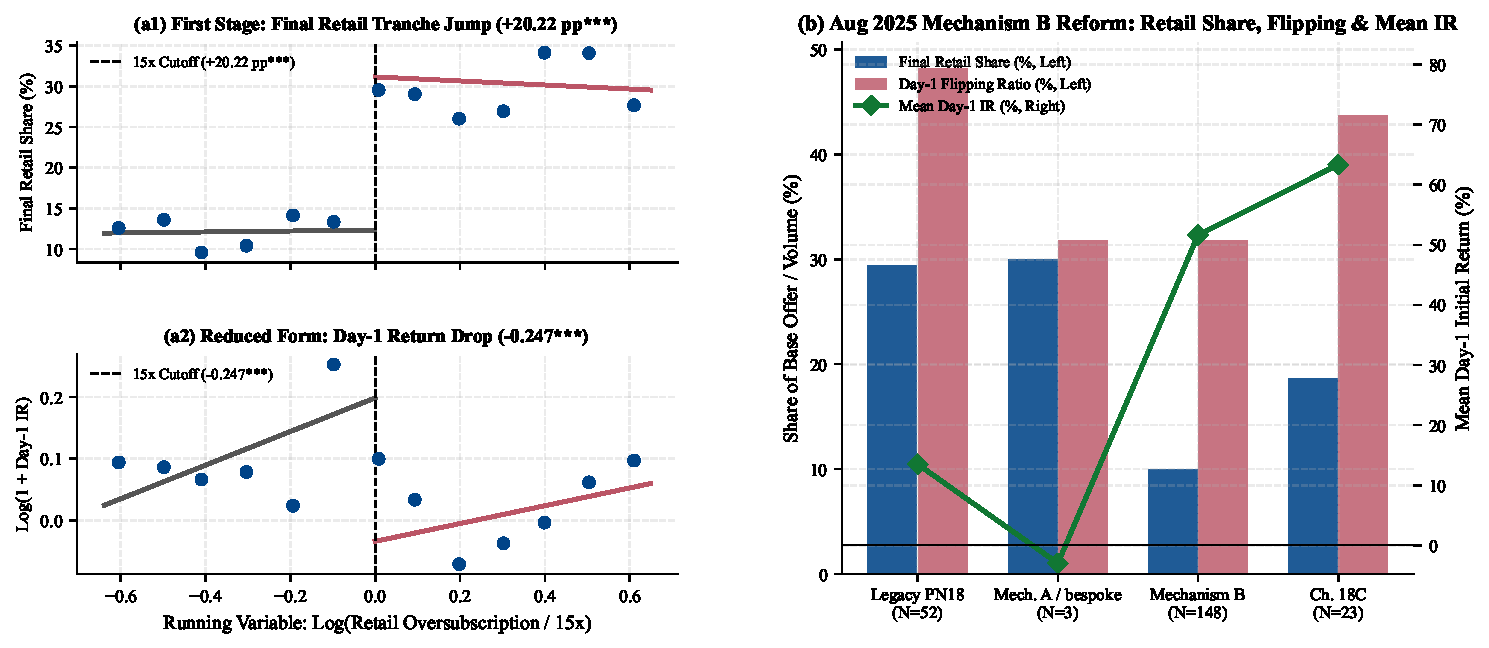
\includegraphics[width=0.92\textwidth]{../overview_paper/figures/journal_fig6.pdf}
\caption{PN18 15x regression discontinuity jumps in final retail allocation and Day-1 log returns (1998--2025.07), alongside retail share, flipping, and mean initial returns across 2025--2026Q3 statutory allocation regimes ($N = 226$).}
\end{figure}

\vspace{6pt}
\begin{figure}[p]
\centering
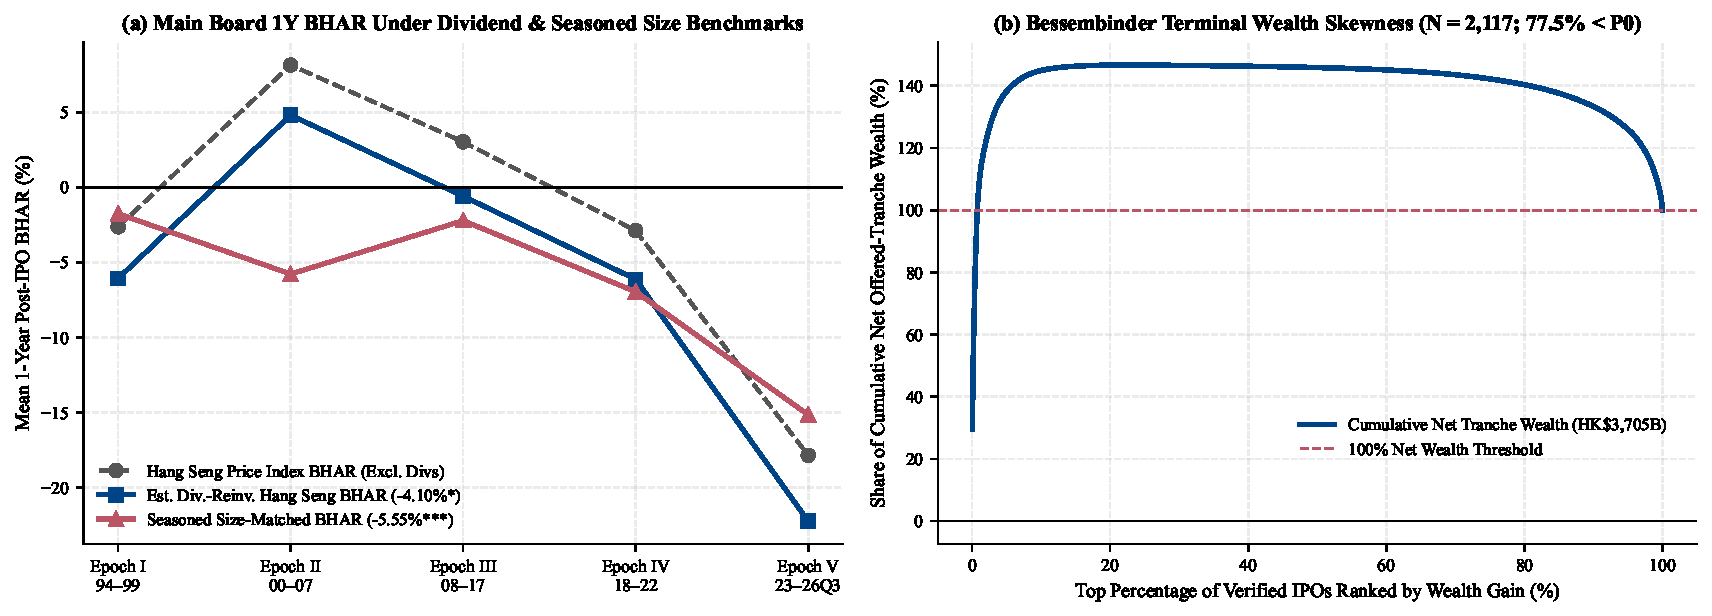
\includegraphics[width=0.92\textwidth]{../overview_paper/figures/journal_fig8.pdf}
\caption{Five-epoch Main Board one-year buy-and-hold abnormal returns across price-HSI, dividend-reinvested HSI-TR, and size-matched benchmarks (Panel a), and Bessembinder cumulative offered-tranche wealth concentration across 2,117 split-verified IPOs (Panel b).}
\end{figure}

\end{document}
